%https://docs.google.com/presentation/d/1ZPpSvbp0xC4q1KGkntliPrwuhJng65D7QPWC9apuXjw/edit?usp=sharing

%! TEX program = lualatex

\documentclass[nobackground,dvipsnames,table]{beamer}
\usepackage{tsc}
\usepackage{pdfpc}
\usepackage{pgfpages}
\usepackage{multimedia}

\mode<presentation>
{\usetheme{default}
	\usecolortheme{tsc}
	\setbeamercovered{transparent}
	\useinnertheme[shadow=false]{rounded}
	\usebackgroundtemplate{}
	\setbeamercolor*{frametitle}{parent=palette primary}
	\setbeamerfont{block title}{size={}}
	\setbeamertemplate{navigation symbols}{}
    \setbeamertemplate{itemize items}[circle]
    \setbeamertemplate{enumerate items}[circle]
}
%%%%%%%% edit hyperlink colors %%%%%%%%
\hypersetup{
  colorlinks   = true, 
  urlcolor     = tscurl, % color of external hyperlinks
  linkcolor    = white,   % color of internal links
}
%%% below command addresses log output error when trying to use \\ in \author %%%
\pdfstringdefDisableCommands{%
  \def\\{}%
}

\title[Terorrism, Radicalization, and Extremism]{Terorrism, Radicalization, and Extremism}
%\subtitle{A document made with thought and care}

\author[]{\scriptsize{Mariana Olaizola Rosenblat (NYU Stern Center for Business and Human Rights)
\\ Inga Kristina Trauthig (The University of Texas at Austin)}}
%\institute[TSC]{\large Trust \& Safety Teaching Consortium}
\date[]{}
\subject{Trust and Safety}

\AddToShipoutPictureBG*{
  \AtPageLowerLeft{\hspace{-0.4cm}
    
\includegraphics[width=13.1cm]{img/consortium-image}}
}
% Change this to make a file with just slides, just notes or both
%\setbeameroption{hide notes}                 % Only slides
%\setbeameroption{show only notes}            % Only notes
\setbeameroption{show notes on second screen} % Both

\begin{document}

%\coverpage

%%%%%%%%%%%%%%%%%%%%%%%%%%%%%%%%%%%%%%%%%%%%%%%%
%%%%%%%%%%%%%%%%  SLIDE 1  %%%%%%%%%%%%%%%%%%%%%
%%%%%%%%%%%%%%%%%%%%%%%%%%%%%%%%%%%%%%%%%%%%%%%%
\begin{frame}
	\titlepage
\end{frame}

%%%%%%%%%%%%%%%%%%%%%%%%%%%%%%%%%%%%%%%%%%%%%%%%
%%%%%%%%%%%%%%%%  SLIDE 2  %%%%%%%%%%%%%%%%%%%%%
%%%%%%%%%%%%%%%%%%%%%%%%%%%%%%%%%%%%%%%%%%%%%%%%
\begin{frame}{Learning Objectives}

Today we will:
\begin{itemize}
    \item Understand the concepts of terrorism, extremism and radicalization in relation to the online space.
    \item Explore existing and potential future ways of countering online extremism.
    \item Analyze the role online platforms play in facilitating extremist activity by examining two case studies: the January 6th insurrection at the US Capitol and in gaming sites.
\end{itemize}
\end{frame}

%%%%%%%%%%%%%%%%%%%%%%%%%%%%%%%%%%%%%%%%%%%%%%%%
%%%%%%%%%%%%%%%%  SLIDE 3  %%%%%%%%%%%%%%%%%%%%%
%%%%%%%%%%%%%%%%%%%%%%%%%%%%%%%%%%%%%%%%%%%%%%%%
\begin{frame}{Framing questions}
\small{
\begin{itemize}
    \item How is extremism related to, and different from, online hate speech?
    \item Is the removal of extremist content from the Internet an effective measure to counter extremism?
    \item What are the benefits and drawbacks of using AI to counter extremism?
    \item How does extremists’ use of encrypted messaging platforms impact the effectiveness of available counter-extremism tools?
    \item How can law shape online platforms’ response to online extremism, and what are law’s limitations?  
    \item What should be the roles of the private and public sectors, respectively, in countering extremism and terrorism online?
    \item How will emerging technologies, such as “the DWeb” and “metaverse” change the ways that extremists exploit online platforms?
\end{itemize}
}
\end{frame}

%%%%%%%%%%%%%%%%%%%%%%%%%%%%%%%%%%%%%%%%%%%%%%%%
%%%%%%%%%%%%%%%%  SLIDE 4  %%%%%%%%%%%%%%%%%%%%%
%%%%%%%%%%%%%%%%%%%%%%%%%%%%%%%%%%%%%%%%%%%%%%%%
\begin{frame}{Defining “extremism”}
\begin{center}
    Relativistic definition: a belief system that lies outside the bounds of currently acceptable/mainstream norms of society. Context-dependent (Neumann)
\end{center}

\begin{center}
    vs.
\end{center}

\begin{center}
    Non-relativistic definition: a belief system held together by an unwavering hostility towards a specific “out-group.” Focused on inter-group hostility (Berger)
\end{center}

\note[]{
Bottom line: No universally accepted definition of extremism. Some convergence among academics (see Charlie Winter et al., “Online Extremism: Research'') \newline 


No internationally binding treaty or customary international norm defining extremism (\url{https://www.uscirf.gov/sites/default/files/Legislation\%20Factsheet\%20-\%20Extremism_0.pdf}).
}
\end{frame}


%%%%%%%%%%%%%%%%%%%%%%%%%%%%%%%%%%%%%%%%%%%%%%%%
%%%%%%%%%%%%%%%%  SLIDE 5.1  %%%%%%%%%%%%%%%%%%%%%
%%%%%%%%%%%%%%%%%%%%%%%%%%%%%%%%%%%%%%%%%%%%%%%%
\begin{frame}{Defining “terrorism”}
\begin{center}
    Behavior-focused definition: “premeditated, politically motivated violence perpetrated against non-combatant targets by sub-national groups or clandestine agents” (US Dept of State)
\end{center}

\begin{center}
    vs. 
\end{center}

\begin{center}
    Belief-focused definition: “a doctrine about the presumed effectiveness of a special form or tactic of fear-generating, coercive political violence” (Schmid)
\end{center}

\note[]{
\tiny{
[Feel free to add others!]\newline 

National governments employ different definitions, some of them quite problematic. E.g.:
\begin{itemize}
    \tiny{
    \item US: Terrorism is defined in Title 22 Chapter 38 U.S. Code § 2656f(d), for purposes of the State Department’s annual country reports on terrorism, as “premeditated, politically motivated violence perpetrated against noncombatant targets by subnational groups or clandestine agents.”
    
    \begin{itemize}
        \tiny{
        \item FBI differentiates between international and domestic terrorism;
        \item USAID defines violent extremism as “advocating, engaging in, preparing, or otherwise supporting ideologically motivated or justified violence to further social, economic, and political objectives.”
        }
    \end{itemize}
    \item UK: Terrorism is an action or threat designed to influence the government or intimidate the public. Its purpose is to advance a political, religious or ideological cause (UK Terrorism Act 2006). 

    \begin{itemize}
        \tiny{\item “Extremism is the vocal or active opposition to our fundamental values, including democracy, the rule of law, individual liberty, and respect and tolerance for different faiths and beliefs. We also regard calls for the death of members of our armed forces as extremist” (UK The Counter Extremism Strategy 2015)}
    \end{itemize}
    \item Russia: “terrorism shall mean the ideology of violence and the practice of influencing the adoption of a decision by public authorities, local self-government bodies or international organizations connected with frightening the population and (or) other forms of unlawful violent actions”. 

    \begin{itemize}
        \tiny{\item A terrorism act can mean the “popularisation of terrorist ideas, dissemination of materials or information urging terrorist activities…” (Counteraction Against Terrorism Law of March 2006)
        \item Any court may add texts to the Federal List of Extremist Materials. As of January 2019, there were over 4,000 items on this list, including many religious texts with no apparent connections to militancy. The list includes the translation of the Bible used by the Jehovah’s Witnesses, which in 2017 was the first centralized religious organization to be banned as an extremist organization in the country.
}
    \end{itemize}
    }
\end{itemize}

}
}
\end{frame}

%%%%%%%%%%%%%%%%%%%%%%%%%%%%%%%%%%%%%%%%%%%%%%%%
%%%%%%%%%%%%%%%%  SLIDE 5.2  %%%%%%%%%%%%%%%%%%%
%%%%%%%%%%%%%%%%%%%%%%%%%%%%%%%%%%%%%%%%%%%%%%%%
\begin{frame}{Defining “terrorism”}
\begin{center}
    Behavior-focused definition: “premeditated, politically motivated violence perpetrated against non-combatant targets by sub-national groups or clandestine agents” (US Dept of State)
\end{center}

\begin{center}
    vs. 
\end{center}

\begin{center}
    Belief-focused definition: “a doctrine about the presumed effectiveness of a special form or tactic of fear-generating, coercive political violence” (Schmid)
\end{center}

\note[]{
\textbf{NOTE: duplicate slide to make space for notes}
\tiny{
\begin{itemize}
    \tiny{
    \item Tajikistan: the extremism law punishes “extremist, terrorist, or revolutionary activities” without requiring acts that involve violence or incitement of imminent violence.
    
    \begin{itemize}
        \tiny{
        \item Trials under these charges lack due process and procedural safeguards. The Tajik government uses concerns over Islamist extremism to justify actions against participants in certain religious or political activities.
        }
    \end{itemize}
    \item Saudi Arabia: the 2014 counterterrorism law and related legislation criminalized as terrorism virtually all forms of peaceful dissent. Terrorism also included calling into question the fundamentals of Islam. 

    \begin{itemize}
        \tiny{\item While the counterterrorism law was amended in 2017 to address some of the human rights concerns by referencing the use of violence as one possible aspect of terrorism, the law still contains overly broad definitions and continues to be applied against activists.}
    \end{itemize}
    \item China: Legislation applicable in Xinjiang province identifies 15 types of behavior the government views as extremist, such as wearing an “abnormal” beard, wearing a veil, or following halal practices (Muslim dietary laws).
    }
\end{itemize} 

***Counter-extremism measures taken by states must be consistent with international human rights standards on, e.g., freedom of religion or belief, freedom of opinion and expression, and the freedom of peaceful assembly and association. Under IHRL, each of these rights can be limited only in very narrow circumstances. Any restrictions need to conform with standards of legality, legitimacy, necessity and proportionality

\url{https://www.uscirf.gov/sites/default/files/Legislation\%20Factsheet\%20-\%20Extremism_0.pdf}
}
}
\end{frame}


%%%%%%%%%%%%%%%%%%%%%%%%%%%%%%%%%%%%%%%%%%%%%%%%
%%%%%%%%%%%%%%%%  SLIDE 6  %%%%%%%%%%%%%%%%%%%%%
%%%%%%%%%%%%%%%%%%%%%%%%%%%%%%%%%%%%%%%%%%%%%%%%
\begin{frame}{Defining “radicalization”}

\begin{center}
    “A process leading towards the increased use of political violence” (della Porta and La Free) \newline 

    “Change in beliefs, feelings, and behaviors in directions that increasingly justify intergroup violence and demand sacrifice in defense of the group” (McCauley and Moskalenko) \newline 

    “The set of processes that causes attitudinal change that leads towards the use of violence” (Neumann and Rogers)
\end{center}

\note[]{
See Charlie Winter et al., “Online Extremism: Research Trends in Internet Activism, Radicalization, and Counter-Strategies,” International Journal of Conflict and Violence, Vol. 14 (2020) \url{https://www.ijcv.org/index.php/ijcv/article/view/3809}
}
\end{frame}


%%%%%%%%%%%%%%%%%%%%%%%%%%%%%%%%%%%%%%%%%%%%%%%%
%%%%%%%%%%%%%%%%  SLIDE 7  %%%%%%%%%%%%%%%%%%%%%
%%%%%%%%%%%%%%%%%%%%%%%%%%%%%%%%%%%%%%%%%%%%%%%%
\begin{frame}{10-minute exercise}
Turn to the person next to you. In pairs, draft workable definitions for (1) extremism and (2) terrorism for your fictional online platform’s community standards. \newline \newline 

Use examples to illustrate the types of content and behavior you are seeking to prohibit on the platform.

\note[]{[Alternative exercise: have groups look up and critique Facebook’s community guidelines on extremism and terrorism]}
\end{frame}


%%%%%%%%%%%%%%%%%%%%%%%%%%%%%%%%%%%%%%%%%%%%%%%%
%%%%%%%%%%%%%%%%  SLIDE 8  %%%%%%%%%%%%%%%%%%%%%
%%%%%%%%%%%%%%%%%%%%%%%%%%%%%%%%%%%%%%%%%%%%%%%%
\begin{frame}{Dominant strains of extremism online}

\begin{itemize}
    \item Radical Islamists and Salafi-jihadis
    \item Far-right extremists, alt-right, white supremacists
    \item Manosphere, incelosphere
    \item Left-wing extremists, sometimes focused on environmental issues \newline 
\end{itemize}

(There is overlap as well as reciprocal radicalization between all of them)
\end{frame}


%%%%%%%%%%%%%%%%%%%%%%%%%%%%%%%%%%%%%%%%%%%%%%%%
%%%%%%%%%%%%%%%%  SLIDE 9.1  %%%%%%%%%%%%%%%%%%%%%
%%%%%%%%%%%%%%%%%%%%%%%%%%%%%%%%%%%%%%%%%%%%%%%%
\begin{frame}{\emph{Why} do extremists use the Internet?}

\begin{minipage}[b]{0.4\textwidth}
    \raggedright % not sure if this does anything; tried to adjust spacing
    \small{
    \begin{itemize}
    \footnotesize{
        \item Disseminate ideology
        \item Increase global recognition and appeal
        \item Produce and publish propaganda
        \item Mine sensitive data
        \item Recruit and indoctrinate members
        %\item Build up organizational structure and nurture future leaders
        %\item Share information, including strategic and tactical advice 
        %\item Socialize and network with like-minded people and groups
        %\item Plan, coordinate and mobilize for attacks
        %\item Fundraise 
        }
    \end{itemize} 
    }
\end{minipage}
\hfill

\includegraphics[scale=0.3]{img/fig1.jpg}

\note[]{Pic from google with creative commons license}
\end{frame}

%%%%%%%%%%%%%%%%%%%%%%%%%%%%%%%%%%%%%%%%%%%%%%%%
%%%%%%%%%%%%%%%%  SLIDE 9.2  %%%%%%%%%%%%%%%%%%%%%
%%%%%%%%%%%%%%%%%%%%%%%%%%%%%%%%%%%%%%%%%%%%%%%%
\begin{frame}{\emph{Why} do extremists use the Internet?}

\begin{minipage}[b]{0.4\textwidth}
    \raggedright % not sure if this does anything; tried to adjust spacing
    \small{
    \begin{itemize}
    \footnotesize{
        %\item Disseminate ideology
        %\item Increase global recognition and appeal
        %\item Produce and publish propaganda
        %\item Mine sensitive data
        %\item Recruit and indoctrinate members
        \item Build up organizational structure and nurture future leaders
        \item Share information, including strategic and tactical advice 
        \item Socialize and network with like-minded people and groups
        \item Plan, coordinate and mobilize for attacks
        \item Fundraise 
        }
    \end{itemize} 
    }
\end{minipage}
\hfill

\includegraphics[scale=0.3]{img/fig1.jpg}

\note[]{Pic from google with creative commons license}
\end{frame}


%%%%%%%%%%%%%%%%%%%%%%%%%%%%%%%%%%%%%%%%%%%%%%%%
%%%%%%%%%%%%%%%%  SLIDE 10  %%%%%%%%%%%%%%%%%%%%%
%%%%%%%%%%%%%%%%%%%%%%%%%%%%%%%%%%%%%%%%%%%%%%%%
\begin{frame}{\emph{How} do extremists use the Internet?}

\raisebox{6.5ex}{
\begin{minipage}[]{0.4\textwidth}
    \raggedright % not sure if this does anything; tried to adjust spacing
    \small{
    \begin{itemize}
    \footnotesize{
        \item Extremists rely on different platforms (fringe, mainstream, encrypted) for different reasons (audience reach vs. security, for example), and platform migration is common.
        \item E.g., in early 2023, far-right actors migrated from Telegram to TamTam, and in 2016 ISIS supported moved from Twitter to Telegram.
        }
    \end{itemize} 
    }
\end{minipage}
}
\hfill

\includegraphics[scale=0.3]{img/fig2.jpg}

\note[]{Pic from this report: \url{https://crestresearch.ac.uk/resources/how-telegram-disruption-impacts-jihadist-platform-migration/}}
\end{frame}


%%%%%%%%%%%%%%%%%%%%%%%%%%%%%%%%%%%%%%%%%%%%%%%%
%%%%%%%%%%%%%%%%  SLIDE 11  %%%%%%%%%%%%%%%%%%%%%
%%%%%%%%%%%%%%%%%%%%%%%%%%%%%%%%%%%%%%%%%%%%%%%%
\begin{frame}{Countering online extremism - the role of platforms}
Reactive/defensive measures:
\begin{itemize}
    \item Content removal
    \item Account suspensions
    \item Counter-speech / counter-activism \newline 
\end{itemize}

Proactive/offensive measures:
\begin{itemize}
    \item Counter-messaging
    \item Awareness-raising / education 
\end{itemize}

\note[]{Discuss pros and cons.}
\end{frame}


%%%%%%%%%%%%%%%%%%%%%%%%%%%%%%%%%%%%%%%%%%%%%%%%
%%%%%%%%%%%%%%%%  SLIDE 12  %%%%%%%%%%%%%%%%%%%%%
%%%%%%%%%%%%%%%%%%%%%%%%%%%%%%%%%%%%%%%%%%%%%%%%
\begin{frame}{Technological approaches: AI}
\footnotesize{
Challenges:
\begin{itemize}
    \footnotesize{
    \item Generative AI apps like Chat-GPT increase the speed and ease of generating extremist disinformation. 
    \item Deepfakes and other synthetic media enable the creation of propaganda materials that can be used in social media disinformation campaigns to manipulate public opinion.
    }
\end{itemize}

Opportunities/solutions:
\begin{itemize}
    \footnotesize{
    \item AI models can be trained to spot AI-manipulated audio-visual content.
    \item Large hash (digital fingerprint) databases are used to scan online services for matching terrorist content in real time and a high scale.
    \item Artificial data produced by general adversarial networks (GANs) can also be used to train algorithms.
    \item Social network analysis (SNA) can be used for understanding and modelling network structures and identifying the main actors or groups therein.
    }
\end{itemize}
}

\note[]{Open-source databases on terrorism, such as the Global Terrorism Database and GIFCT hash database, can be used for the purposes of training algorithms. \newline 

In December 2016, Facebook, Twitter, Google and Microsoft announced plans to tackle extremist content such as terrorist recruitment videos and violent terrorist imagery using PhotoDNA (previously used to identify CSAM)

}

\end{frame}


%%%%%%%%%%%%%%%%%%%%%%%%%%%%%%%%%%%%%%%%%%%%%%%%
%%%%%%%%%%%%%%%%  SLIDE 13  %%%%%%%%%%%%%%%%%%%%%
%%%%%%%%%%%%%%%%%%%%%%%%%%%%%%%%%%%%%%%%%%%%%%%%
\begin{frame}{Human rights risks of AI deployment}
\begin{itemize}
    \item Privacy risks
    \item Infringement on freedom of thought and freedom of association
    \begin{itemize}
        \item Especially when takedowns are mandated by public authorities.
        \item Lack of clear and adequate definitions of extremism and terrorism in many legal systems allows these terms to be weaponized to crack down on political opponents.
    \end{itemize}
    \item Discrimination
    \begin{itemize}
        \item Bias in data fed to algorithms results in discriminatory AI. \newline \newline 
    \end{itemize}
\end{itemize}

Other reminders / cautionary notes about AI:
\begin{itemize}
    \item Lack of consensus definitions of extremism and terrorism, respectively, can lead to fragmented data collection.
\end{itemize}

\note[]{\footnotesize{The mass and indiscriminate collection of data online in order to gather intelligence carries inherent privacy risks. Need proper safeguards on storage and use. \newline 

Without a clear and narrow definition of illegal extremist and terrorist content, enforced takedowns and other punitive actions can infringe on freedom of expression and thought.  (\emph{“law enforcement and counter-terrorism agencies aiming to use AI-enabled technologies to direct users at risk of radicalization to counter-narrative content need to consider the possibility that these technologies could result in unlawful interference with the right to freedom of thought through the manipulation of the way that the targeted users think”}). \newline 

Targeting individuals for differential treatment based on protected characteristics contravenes right to non-discrimination. AI-enabled systems can discriminate against vulnerable groups by screening for indicators that act as proxies for protected characteristics. }
}
\end{frame}


%%%%%%%%%%%%%%%%%%%%%%%%%%%%%%%%%%%%%%%%%%%%%%%%
%%%%%%%%%%%%%%%%  SLIDE 14.1  %%%%%%%%%%%%%%%%%%%%%
%%%%%%%%%%%%%%%%%%%%%%%%%%%%%%%%%%%%%%%%%%%%%%%%
\begin{frame}{Countering online extremism – The role of law/regulation}

\small{
EU Rules on Terrorist Content Online (\href{https://eur-lex.europa.eu/legal-content/EN/TXT/HTML/?uri=CELEX:32021R0784\&from=EN}{2021/784})

\begin{itemize}
    \small{
    \item Since June 2022, all tech companies offering their services in the EU are required to take action against terrorist content found on their platforms. 
    \item Hosting service providers must remove terrorist content within one hour of receiving a removal order issued by competent authorities.
    \item Internet platforms that do not systematically comply with the rules are liable to be fined up to 4% of their global turnover. 
    \item Resources: \href{https://tate.techagainstterrorism.org/about}{Tech Against Terrorism Europe} (TATE) provides a free, bespoke and comprehensive programme of support to hosting service providers to ensure to compliance with the regulations.
    }
\end{itemize}

}
\note[]{Europe has been a leader in advancing online platform regulation.}
\end{frame}


%%%%%%%%%%%%%%%%%%%%%%%%%%%%%%%%%%%%%%%%%%%%%%%%
%%%%%%%%%%%%%%%%  SLIDE 14.2  %%%%%%%%%%%%%%%%%%%%%
%%%%%%%%%%%%%%%%%%%%%%%%%%%%%%%%%%%%%%%%%%%%%%%%
\begin{frame}{Countering online extremism – The role of law/regulation}
\small{
EU Digital Services Act
\begin{itemize}
    \small{
    \item As of November 2022, online platforms are required to remove content that is illegal in any EU Member State, suspend accounts that disseminate illegal content---including hate speech, terrorist content, child sexual abuse material, and disinformation---and report criminal behavior.
    \item Very large online platforms need to produce an annual risk assessment and undergo an independent audit, have risk mitigation measures in place, and appoint a compliance officer for illegal content obligations. 
    }
\end{itemize}
}
\note[]{Europe has been a leader in advancing online platform regulation.}
\end{frame}

%%%%%%%%%%%%%%%%%%%%%%%%%%%%%%%%%%%%%%%%%%%%%%%%
%%%%%%%%%%%%%%%%  SLIDE 15  %%%%%%%%%%%%%%%%%%%%%
%%%%%%%%%%%%%%%%%%%%%%%%%%%%%%%%%%%%%%%%%%%%%%%%
\begin{frame}{Countering online extremism – The role of law/regulation II}
US Anti-Terrorism Act (ATA) \newline \newline 
Justice Against Sponsors of Terrorism Act (JASTA)\newline \newline 
\textbf{Does Section 230 of the Communications Decency Act exempt online platforms from liability when they algorithmically promote terrorist content?}\newline \newline 
Supreme Court cases (decision pending)
\begin{itemize}
    \item \emph{Gonzalez v. Google LLC}
    \item \emph{Twitter, Inc. v. Taamneh}
\end{itemize}
\note[]{The US federal govt doesn’t (yet) regulate online platforms directly. }
\end{frame}

%%%%%%%%%%%%%%%%%%%%%%%%%%%%%%%%%%%%%%%%%%%%%%%%
%%%%%%%%%%%%%%%%  SLIDE 16  %%%%%%%%%%%%%%%%%%%%%
%%%%%%%%%%%%%%%%%%%%%%%%%%%%%%%%%%%%%%%%%%%%%%%%
\begin{frame}{How anti-extremism laws can be weaponized \emph{against} human rights}

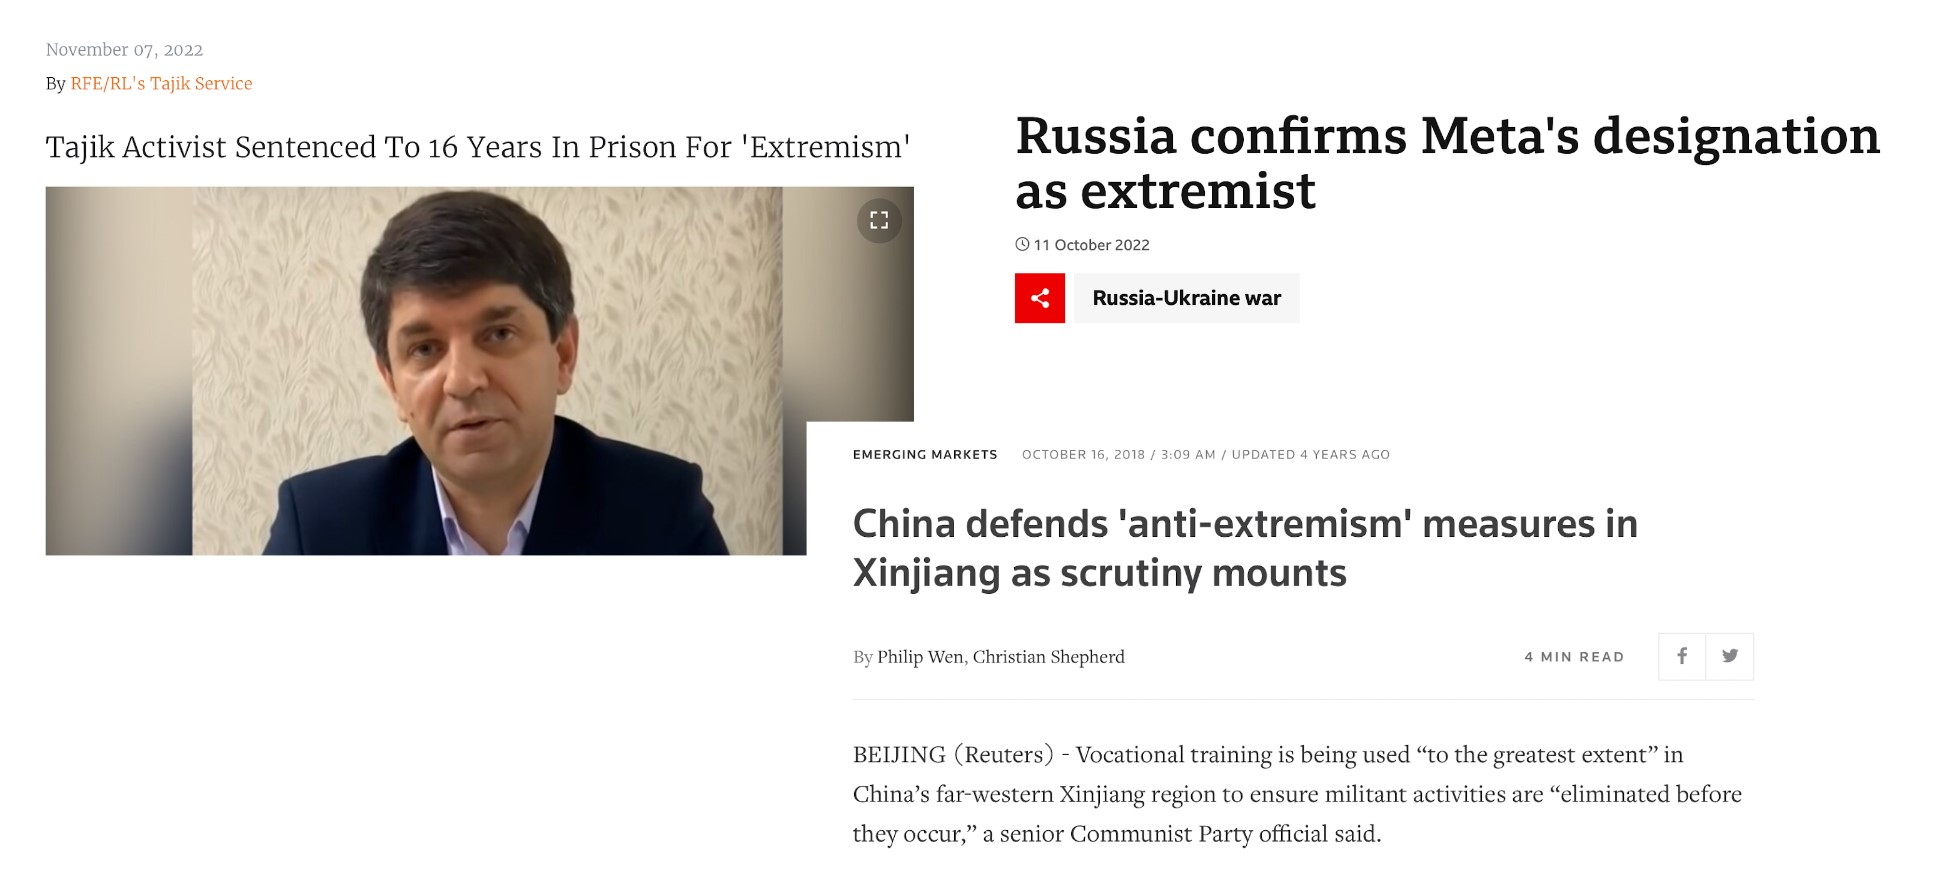
\includegraphics[scale=0.27]{img/fig3.jpg}

\note[]{
A few examples from Russia, Tajikistan, China.

\begin{itemize}
    \item China: Legislation applicable in Xinjiang province identifies 15 types of behavior the government views as extremist, such as wearing an “abnormal” beard, wearing a veil, or following halal practices (Muslim dietary laws).
    \item Tajikistan: the extremism law punishes “extremist, terrorist, or revolutionary activities” without requiring acts that involve violence or incitement of imminent violence. Law has been used to punish political opposition. 
    \item Russia: following its invasion of Ukraine, Russia designated Facebook as an extremist org because Facebook wouldn’t comply with Russian gov commands.
\end{itemize}
}
\end{frame}


%%%%%%%%%%%%%%%%%%%%%%%%%%%%%%%%%%%%%%%%%%%%%%%%
%%%%%%%%%%%%%%%%  SLIDE 17  %%%%%%%%%%%%%%%%%%%%%
%%%%%%%%%%%%%%%%%%%%%%%%%%%%%%%%%%%%%%%%%%%%%%%%
\begin{frame}{Case study: Jan 6 insurrection}
\begin{itemize}
    \item What role did online platforms play in the January 6th storming of the Capitol?
    \item Are companies and law enforcement (better) prepared to confront similar threats today?
\end{itemize}

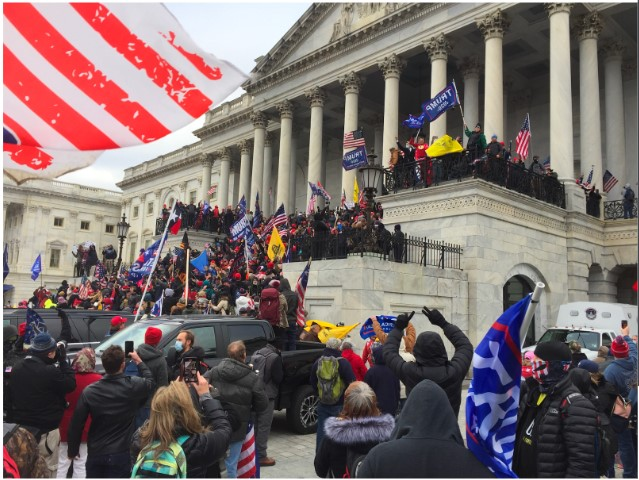
\includegraphics[width=.49\textwidth]{img/fig6.jpg}

\includegraphics[width=.49\textwidth]{img/fig5.jpg}

\note[]{Right corner picture: Taken from report “The WOmen of Jan 6th” by the Program of Extremism in DC: \url{https://extremism.gwu.edu/sites/g/files/zaxdzs2191/f/Women-of-Jan6_Matfess-and-Margolin.pdf}}
\end{frame}


%%%%%%%%%%%%%%%%%%%%%%%%%%%%%%%%%%%%%%%%%%%%%%%%
%%%%%%%%%%%%%%%%  SLIDE 18  %%%%%%%%%%%%%%%%%%%%%
%%%%%%%%%%%%%%%%%%%%%%%%%%%%%%%%%%%%%%%%%%%%%%%%
\begin{frame}{Case study: Online gaming}

\begin{itemize}
    \item Why is online gaming an attractive forum for extremists?
    \item How can the gaming industry better respond to extremist exploitation of gaming platforms? 
\end{itemize}


\includegraphics[width=\textwidth]{img/fig4.jpg}

\note[]{Screenshots taken by NYU Stern Center for Business and Human Rights. \newline \newline 
Top left: screenshot of ISIS propaganda videos created by the 16-year-old Singaporean teenager using Roblox game footage.\newline \newline 
Bottom left: neo-Nazi username in Call of Duty leaderboard. \newline \newline 
Bottom right: Nazi village on Roblox.}
\end{frame}



%%%%%%%%%%%%%%%%%%%%%%%%%%%%%%%%%%%%%%%%%%%%%%%%
%%%%%%%%%%%%%%%%  SLIDE 19  %%%%%%%%%%%%%%%%%%%%%
%%%%%%%%%%%%%%%%%%%%%%%%%%%%%%%%%%%%%%%%%%%%%%%%
\begin{frame}{What next?}
\footnotesize{
DWeb (decentralized web)
\begin{itemize}
\footnotesize{
    \item DWeb technology could be exploited for data storage and retrieval purposes. In that case, “[…] decentralized methods of data storage could make it difficult, if not practically impossible, for a single entity to censor content”
    \item Will this make it impossible for extremist content to be removed and will thus be accessible to anyone who knows where to find it?
    \item Are extremists already relying on Dweb technologies? Which ones and why?
    }
\end{itemize}

Metaverse
\begin{itemize}
\footnotesize{
    \item How will the metaverse enable new forms of extremist and terrorist recruitment, networking and coordination?
    \item How will existing counter-extremism measures fare in an immersive, always-on 3D virtual space?
    \item Who will be responsible for policing the metaverse? 
    \item What proactive steps can industry and government take to prevent and mitigate extremist exploitation of this new expansive virtual realm?}
\end{itemize}
}
\end{frame}

%%%%%%%%%%%%%%%%%%%%%%%%%%%%%%%%%%%%%%%%%%%%%%%%
%%%%%%%%%%%%%%%%  SLIDE 20.1  %%%%%%%%%%%%%%%%%%%%%
%%%%%%%%%%%%%%%%%%%%%%%%%%%%%%%%%%%%%%%%%%%%%%%%
\begin{frame}{Readings / References}
\tiny{
\textbf{5 core readings (other formats like podcasts fine too): }

\begin{enumerate}
    \item \underline{Online extremism and potential countermeasures:} \newline 
Charlie Winter et al., “Online Extremism: Research Trends in Internet Activism, Radicalization, and Counter-Strategies,” \emph{International Journal of Conflict and Violence}, Vol. 14 (2020) \url{https://www.ijcv.org/index.php/ijcv/article/view/3809}
    \item \underline{Overview of suggested solutions in academia:} \newline 
Correa, D., \& Sureka, A. Solutions to detect and analyze online radicalization: a survey. \emph{arXiv preprint arXiv:1301.4916 (2013)}. \url{https://arxiv.org/abs/1301.4916}
    \item \underline{Countering Terrorism Online with Artificial Intelligence:} \newline  
An Overview for Law Enforcement and Counter-Terrorism Agencies in South Asia and South-East Asia, United Nations Office of Counter-Terrorism and United Nations Counter-Terrorism Centre (2021), pp. 10-14, 23-34, 43-49. \url{https://www.un.org/counterterrorism/sites/www.un.org.counterterrorism/files/countering-terrorism-online-with-ai-uncct-unicri-report-web.pdf}
    \item \underline{Social media’s role in the Jan 6th insurrection:} \newline 
Case study – Jen Patja Howell, The Lawfare Podcast: A Jan. 6 Committee Staffer on Social Media and the Insurrection (Feb. 8, 2023) \url{https://www.un.org/counterterrorism/sites/www.un.org.counterterrorism/files/countering-terrorism-online-with-ai-uncct-unicri-report-web.pdf}
    \item \underline{Gaming sites and extremists:} \newline 
“Gaming the System: How Extremists Exploit Gaming Sites and What Can be Done to Stop Them,” NYU Stern Center for Business and Human Rights (forthcoming Mar. 2023).
\end{enumerate}
}
\end{frame}

%%%%%%%%%%%%%%%%%%%%%%%%%%%%%%%%%%%%%%%%%%%%%%%%
%%%%%%%%%%%%%%%%  SLIDE 20.2  %%%%%%%%%%%%%%%%%%%%%
%%%%%%%%%%%%%%%%%%%%%%%%%%%%%%%%%%%%%%%%%%%%%%%%
\begin{frame}{Readings / References}
\tiny{

\textbf{[Optional] Additional readings:} 
\underline{Online extremism outside of main social media platforms/emerging challenges:}
\begin{itemize}
    \tiny{
    \item Lorand Bodo and Inga Kristina Trauthig, “Emergent Technologies and Extremists: The DWeb as a New Internet Reality?” Global Network on Extremism and Technology (July 2022). \url{https://gnet-research.org/wp-content/uploads/2022/07/GNET-Report-Emergent-Technologies-Extremists-Web.pdf}
    \item Elson, Joel S, Doctor, Austin C and Sam Hunter. The metaverse offers a future full of potential - for terrorists and extremists, too. The Conversation (January 7, 2022). \url{https://theconversation.com/the-metaverse-offers-a-future-full-of-potential-for-terrorists-and-extremists-too-173622}
    }
\end{itemize}

\textbf{Additional resources for further readings:}
\begin{itemize}
    \item Center for Countering Digital Hate: \url{https://counterhate.com/}
    \item GIFCT website: \url{https://gifct.org/}
    \item Global Network on Extremism and Technology: \url{https://gnet-research.org/}
    \item ISD Global toolkits: \url{https://www.isdglobal.org/pub-types/toolkits/?fwp_language=english}
    \item Tech Against Terrorism: \url{https://www.techagainstterrorism.org/}
    \item VOX-Pol Network of Excellence (NoE): \url{https://www.voxpol.eu/}
\end{itemize}

}
\end{frame}

%\backpage

\end{document}